%% ****** Start of file aiptemplate.tex ****** %
%%
%%   This file is part of the files in the distribution of AIP substyles for
% %  REVTeX4.
%%   Version 4.1 of 9 October 2009.
%%
%
% This is a template for producing documents for use with
% the REVTEX 4.1 document class and the AIP substyles.
%
% Copy this file to another name and then work on that file.
% That way, you always have this original template file to use.

\documentclass[aip,graphicx]{revtex4-1}
%\documentclass[aip,reprint]{revtex4-1}
\usepackage[draft]{todonotes}
\usepackage{subcaption}

\draft % marks overfull lines with a black rule on the right

\begin{document}

% Use the \preprint command to place your local institutional report number
% on the title page in preprint mode.
% Multiple \preprint commands are allowed.
\preprint{}

\title{Modeling the near-wake of a vertical-axis cross-flow turbine with 2-D and
    3-D RANS}

% repeat the \author .. \affiliation  etc. as needed
% \email, \thanks, \homepage, \altaffiliation all apply to the current author.
% Explanatory text should go in the []'s,
% actual e-mail address or url should go in the {}'s for \email and \homepage.
% Please use the appropriate macro for the type of information

% \affiliation command applies to all authors since the last \affiliation command.
% The \affiliation command should follow the other information.

\author{Peter Bachant}
\email[]{pxl3@unh.edu}
%\homepage[]{Your web page}
%\thanks{}
%\altaffiliation{}
\affiliation{Center for Ocean Renewable Energy, University of New Hampshire,
Durham, NH}

\author{Martin Wosnik}
%\email[]{}
%\homepage[]{Your web page}
%\thanks{}
%\altaffiliation{}
\affiliation{Center for Ocean Renewable Energy, University of New Hampshire,
Durham, NH}

% Collaboration name, if desired (requires use of superscriptaddress option in
% \documentclass).
% \noaffiliation is required (may also be used with the \author command).
%\collaboration{}
%\noaffiliation

\date{\today}

\begin{abstract}
    The near-wake of a vertical-axis cross-flow turbine (CFT) was modeled
    numerically via blade-resolved $k$--$\omega$ SST and Spalart--Allmaras RANS
    models in two and three dimensions. Results for each case are compared with
    experimental measurements of the turbine shaft power, overall drag, mean
    velocity, turbulence kinetic energy, and momentum transport terms in the
    near-wake at one diameter downstream. It was shown that 2-D simulations
    overpredict turbine loading and do not resolve mean vertical momentum
    transport, which plays an important role in the near-wake's momentum
    balance. The 3-D simulations faired better at predicting performance, with
    the Spalart--Allmaras model predictions being closest to the experiments.
    The SST model more accurately predicted the turbulence kinetic energy while
    the Spalart--Allmaras model more closely matched the momentum transport
    terms in the near-wake. These results show the potential of blade-resolved
    RANS as a design tool and a way to ``interpolate'' experimental flow field
    measurements.
\end{abstract}

\pacs{}% insert suggested PACS numbers in braces on next line

\maketitle %\maketitle must follow title, authors, abstract and \pacs
\listoftodos

\section{Introduction}

In the pursuit of a fully sustainable energy profile, cross-flow (often
vertical-axis) turbines (CFTs) can still play a role. Despite extensive research
and development in the 1970s through the early 1990s by groups like Sandia
National Labs in the US \cite{Sutherland2012} and the National Research Council
in Canada \cite{Para2002}, the vertical-axis cross-flow Darrieus turbines were
all but abandoned for large scale commercial terrestrial wind power. Today,
however, with the development of marine hydrokinetic (MHK) energy devices, CFTs
are at the forefront, with the first grid-connected commercial device being a
horizontal-axis CFT manufactured and installed by ORPC in Cobscook Bay, Maine
\cite{ORPC2012}. CFTs are also being examined for small-scale onshore wind in
urban areas \cite{Lott2015}, offshore floating wind farms \cite{Paulsen2011,
    Sandia2012}, and onshore wind farms where power output per unit land area is of
interest \cite{Dabiri2011}.

Despite the development of many simple engineering models based on blade element
momentum or vortex modeling, it remains difficult to predict the performance of
cross-flow turbines in all cases---namely when solidity, or blade chord to
radius ratio is high---a common characteristic of the smaller CFTs. With
computing power becoming evermore available and affordable, computational fluid
dynamics (CFD) presents an attractive method for simulating cross-flow turbines
since it only requires turbulence modeling, i.e., the machine is described from
first principles. However, CFD can be computationally expensive when done in
three dimensions, which may be necessary in some cases. There are many examples
in the literature of 2-D cross-flow turbine simulations with widely varying
results. Balduzzi et al. provides a summary of recent computations and an
attempt to standardize a methodology for using Reynolds-averaged Navier--Stokes
(RANS) to correctly simulate performance of a 2-D CFT \cite{Balduzzi2016}.

Modeling the boundary layer flows on cross-flow turbine blades is very
challenging due to the dynamically changing inflow and angle of attack---which
often exceeds static stall values and causes dynamic stall. Furthermore, the
ability to predict the occurrence and interdependence of boundary layer
transition and separation can have dramatic influence on the blade loading and
therefore the predicted turbine power output. These challenges cast significant
doubt on the ability of high-fidelity CFD modeling to replace wind tunnel or
tank testing of physical models.

\todo[inline]{Put survey of CFD accuracy here}

In this study we set out to model the wake of the University of New Hampshire's
Reference Vertical-Axis (cross-flow) Turbine (UNH-RVAT) using a
Reynolds-averaged Navier--Stokes numerical model. Though studies in the
literature generally focus on predicting the turbine loading and the local blade
boundary layer, we seek to model the larger scale flow produced by the rotor.
The wake of this particular turbine is of interest since it has been shown
experimentally that the near-wake's momentum and energy transport processes are
dominated by vertical advection \cite{Bachant2015-JoT}. It logically follows
that a 2-D simulation would not correctly predict wake recovery, but is of
interest to what extent this is true, since the computational feasibility of 2-D
simulations is attractive.

It is assumed that if the turbine power output and near-wake predictions from
the numerical model match those of the experiments, the flow field can be
inspected in greater detail, i.e., that the experiments will have been
``interpolated''. This will give us access to unmeasured quantities, e.g.
pressure, and allow us to see where the dominant flow structures originate and
help develop low-order wake generator models for use in turbine array modeling.
For example, Shamsoddin and Porte-Agel modeled a 2-D CFT using large eddy
simulation (LES) with an actuator line approach to impart force on the flow
field \cite{Shamsoddin2014}.

To date, little computational work has been done to attempt to design arrays of
CFTs, despite their prospects for closer spacing compared with axial-flow
turbines (AFTs). For example, Araya et al. modeled the flow through a VAT array
using ``leaky Rankine body'' potential flow singularities \cite{Araya2014},
which was able to rank relative performance of array configurations. Goude and
Agren used a 2-D vortex method to simulate a farm of cross-flow turbines
\cite{Goude2010}, though this was not validated with experiments. Durrani et al.
used 2-D CFD to model a group of cross-flow turbines, observing higher power
output for a staggered configuration, but also did not compare with experimental
results \cite{Durrani2011}. Li and Calisal \cite{Li2010} used a 3-D vortex line
method to show mutually improved power output from two adjacent turbines, though
the simulations over-predicted the effects compared with experiments. Antheaume
et al. \cite{Antheaume2008} used a blade element approach coupled with a 3-D
RANS solver to also show how close spacing can improve power output of CFTs.

To summarize, the questions we hope to answer here are:

\begin{enumerate}

    \item Can or should 2-D RANS be used for array design?
    
    \item How accurately can 3-D RANS predict performance?

    \item Can 3-D RANS ``interpolate'' the experimental results and provide insight to develop new low-order wake generators to represent CFTs?

    \item Does 3-D RANS realize the correct proportions of wake recovery
    mechanisms, i.e., are the 3-D blade-resolved results a good ``target'' for
    those from a low-order model?

\end{enumerate}


\section{Turbine description}

In this study we seek to predict the near-wake of the UNH-RVAT turbine, shown in
Figure~\ref{fig:RVAT-CAD}. Experimental performance curves for the UNH-RVAT are
shown in Figure~\ref{fig:exp_perf}. We modeled the turbine at a tip speed ratio
$\lambda=1.9$, which corresponds to the maximum power coefficient, and a turbine
diameter Reynolds number $Re_D \approx 10^6$, which corresponds to a
$Re$-independent state for both performance and near-wake characteristics, as
determined from experimental measurements \cite{Bachant2014,
    Bachant2015-RVAT-Re-dep}.


\begin{figure}[ht]
    \centering
    
    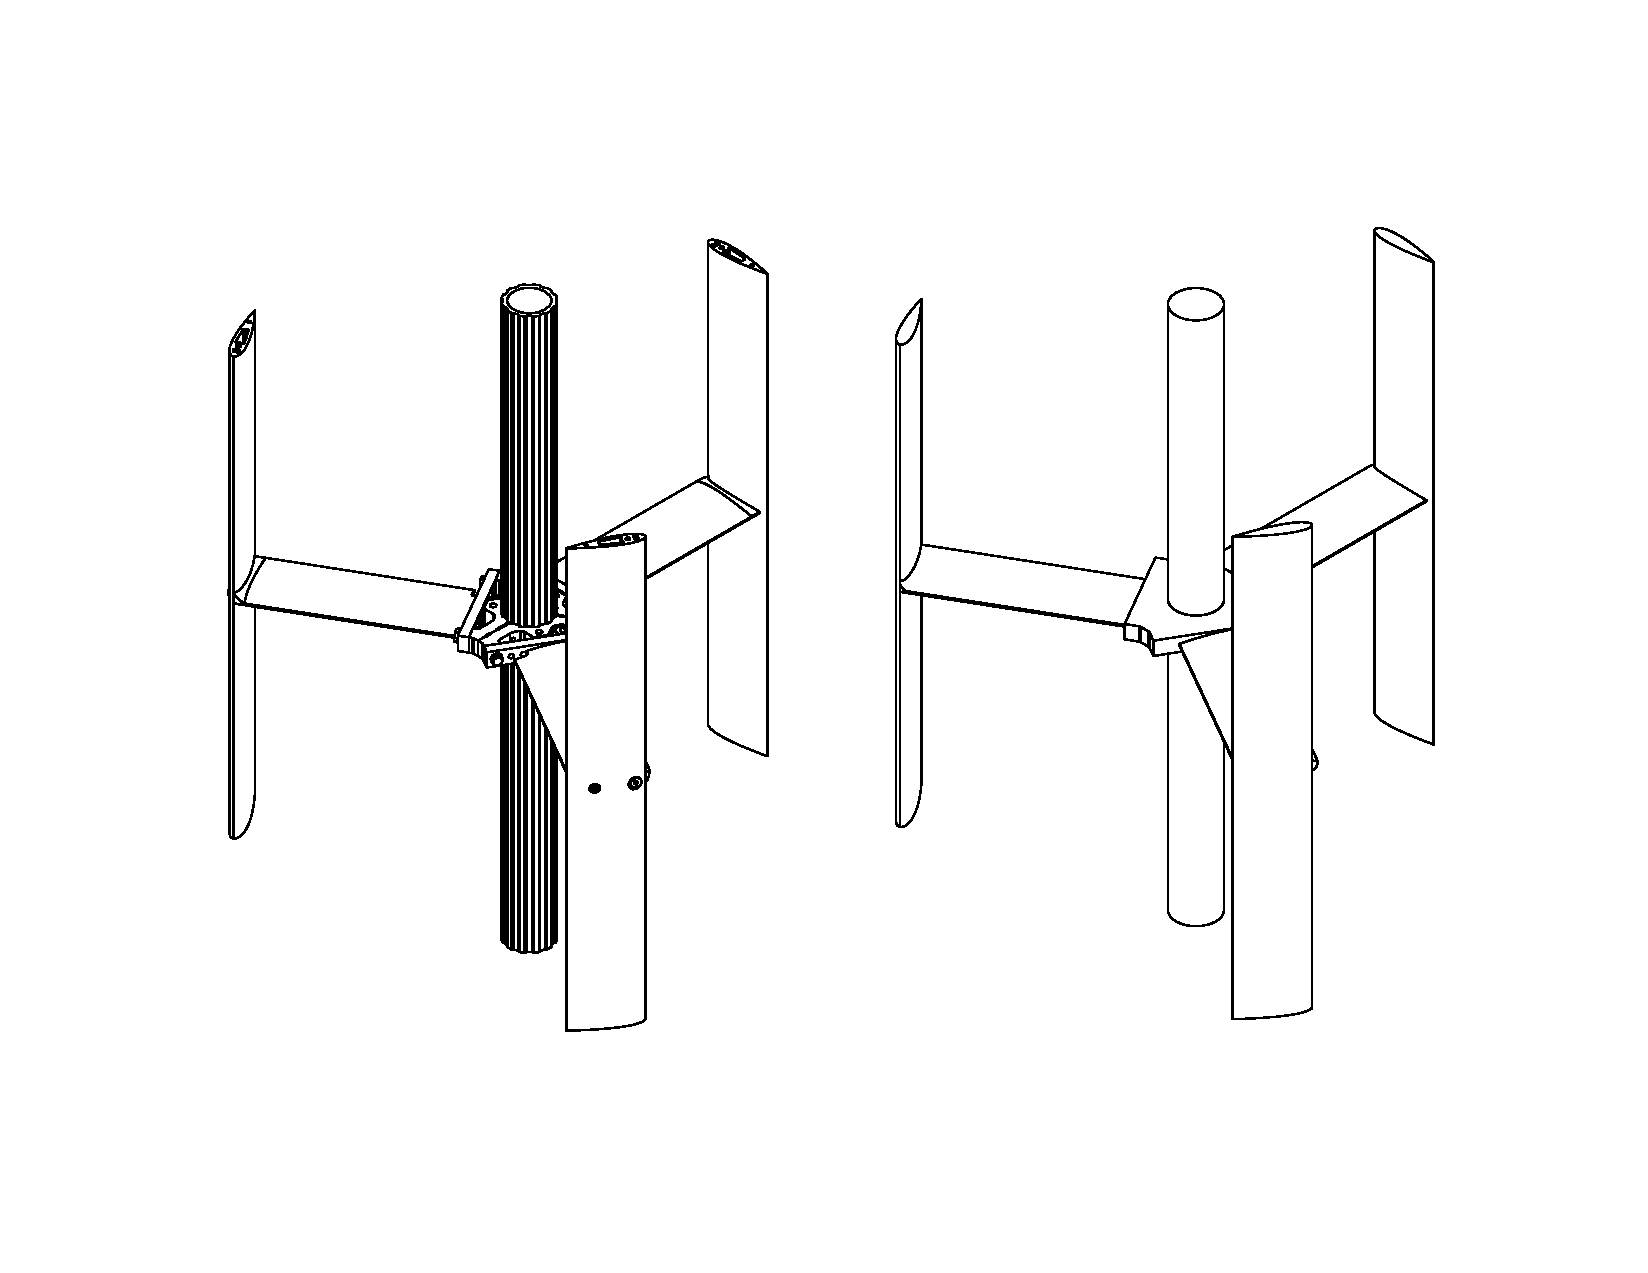
\includegraphics[clip, trim=0 1in 0 1in, width=0.8\textwidth]{figures/CAD}
    
    \caption{CAD drawings of the UNH-RVAT cross-flow turbine as designed (left)
        and cleaned for simulation (right).}
    
    \label{fig:RVAT-CAD}
\end{figure}


\begin{figure}[ht]
    \centering

    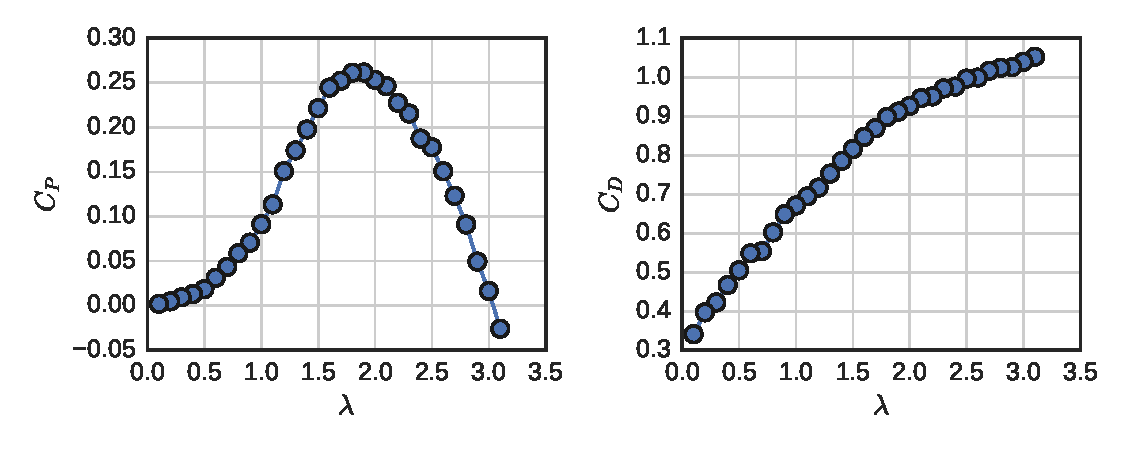
\includegraphics[width=0.9\textwidth]{figures/exp_perf}

    \caption{Mean rotor power (left) and drag (right) coefficient curves from
        the tow tank experiments\cite{Bachant2015-RVAT-Re-dep-data}.}

    \label{fig:exp_perf}
\end{figure}


\section{Numerical models}

The flow field was modeled using the Reynolds-averaged Navier--Stokes equations,
employing two different turbulence models---Menter's $k$--$\omega$ SST
\cite{Menter1994} and the Spalart--Allmaras (SA) one equation model
\cite{Spalart1992}. The SST model was chosen due to its prominence in the
literature for simulating separating flows, which we assumed to be present in
the current problem in the form of dynamic stall. The SA model was shown by
Ferreira et al. \cite{Ferreira2007} to match experimental particle image
velocimetry (PIV) results for a CFT in dynamic stall, though this was a somewhat
low Reynolds number case ($5 \times 10^4$). Further justification for using the
SA model for this case comes from Crivellini and D'Alessandro
\cite{Crivellini2014}, where they successfully modeled the laminar separation
bubble and subsequent boundary layer transition to turbulence at Reynolds
numbers similar to ours.

\subsection{Computational mesh}

The computational domain is a rectangular volume 3.66 m long, 3.66 m wide, and
2.44 m tall (for 3-D), with the turbine located 1.52 m from the inlet, and
centered vertically with a vertical axis. with a cylindrical sliding mesh
interface, where the turbine zone rotates at a mean tip speed ratio
$\lambda=1.9$ with a sinusoidal oscillation at the blade passage
frequency---with and amplitude of 0.19 and the first peak at 0.7 radians---to
mimic the experimental data. The 2-D mesh overview is shown in
Figure~\ref{fig:mesh} and the blade mesh is shown in
Figure~\ref{fig:blade-mesh}.

Meshes were generated using \textit{OpenFOAM}'s \textit{blockMesh} and
\textit{snappyHexMesh} utilities. Mesh topology consists of a background
hexahedral mesh, which is refined in all three directions by a factor of 2 in a
rectangular region containing the turbine and near-wake (0.9 m upstream, 1.3 m
downstream, $\pm 0.9$ m cross-stream, and $\pm 0.8$ m vertically). Cells
adjacent to the turbine shaft and struts are refined by a factor of 4, while
cells adjacent to the blades are refined by a factor of 6. To capture the
boundary layer, 20 layers are added next to the blades with an expansion ratio
of 1.2. Overall mesh refinement is controlled by a single parameter---the number
of cells in the streamwise direction, $N_x$.

3-D computer aided design (CAD) files of the turbine are available from
\cite{Bachant2014-RVAT-CAD}.

\begin{figure}[ht]    
    \includegraphics[width=0.8\textwidth]{figures/2d_mesh}
    
    \caption{Overview of the 2-D computational mesh.}
    
    \label{fig:mesh}
\end{figure}


\begin{figure}[ht]
    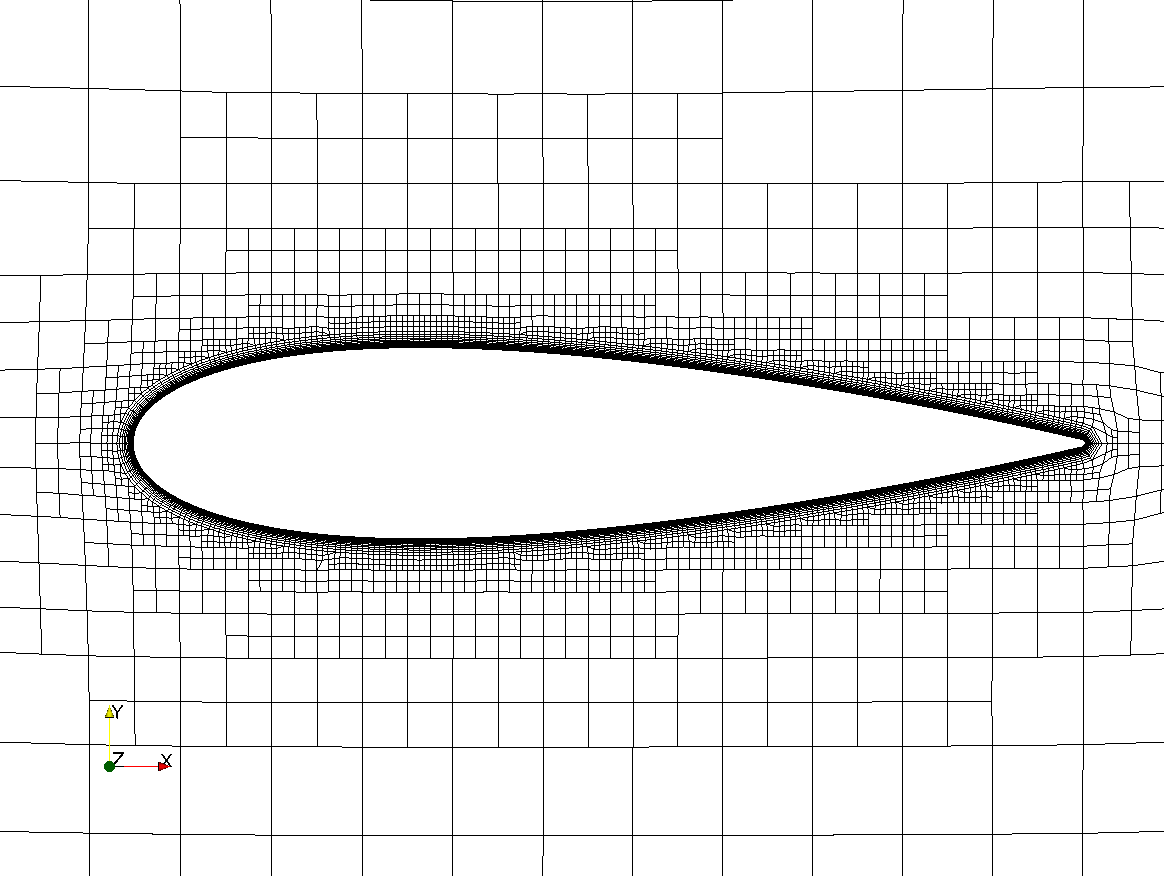
\includegraphics[width=0.7\textwidth]{figures/2D_blade_mesh_closeup}
    
    \caption{Detailed view of the 2-D computational mesh near the blades.}
    
    \label{fig:blade-mesh}
\end{figure}


\subsection{Solver}

Simulations were run using the \textit{pimpleDyMFoam} solver from the
open-source finite volume CFD package \textit{OpenFOAM}, version 2.3.x.
\textit{pimpleDyMFoam} uses a hybrid PISO-SIMPLE algorithm for pressure-velocity
coupling and is compatible with dynamic meshes.

\subsection{Initial and boundary conditions}

Initial and boundary conditions were set to match those of the tow tank as well
as possible. The velocity at the bottom and side walls was fixed to 1 m/s to
match the tow tank case, while the top boundary condition was a slip velocity
condition. Note that in 2-D the top and bottom boundary conditions are
``empty,'' which is an OpenFOAM convention.

\section{Model verification}

The $k$--$\omega$ SST and Spalart--Allmaras RANS model cases were verified for
convergence of the turbine mean power coefficient with respect to grid spacing
and timestep. The grid topology was fixed, but the number of cells per unit
length were scaled proportionally, maintaining the same background mesh cell
aspect ratio. Results for this parameter sweep are shown in
Figure~\ref{fig:verification}, from which the final number of streamwise
grid points $N_x = 70$ was chosen. This corresponds to a total cell count of
approximately $5 \times 10^4$ for the 2-D cases and 16 million for the 3-D case.

\begin{figure}[ht]
    \centering

    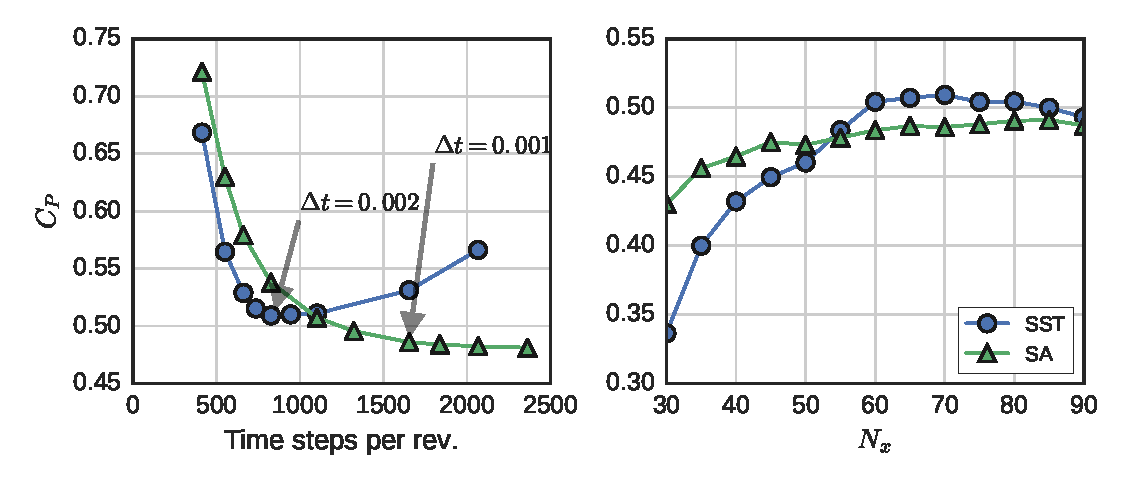
\includegraphics[width=0.9\textwidth]{figures/verification}

    \caption{Time step (left) and grid size (right) dependence for the 2-D case
        with both the SST and SA turbulence models. Time step dependence was carried
        out with $N_x=70$ and grid size dependence with the time steps annotated for
        each turbulence model.}

    \label{fig:verification}
\end{figure}

Time step dependence was studied using the $N_x=70$ grid, the results from which
are shown in Figure~\ref{fig:verification}. It was seen that the
Spalart--Allmaras model converged well with decreasing time step, leading to a
final time step of 0.001 s. The results from the SST model show a local minimum
at $\Delta t = 0.002$ s, with some divergence for smaller time steps. The local
minimum was chosen as the final time step to run the simulations. Note that the
SST model's convergence behavior may be due to its specific implementation in
\textit{OpenFOAM}, and not indicative of the nature of the model equations.
Verification studies for CFTs with this level of detail in the literature are
not common, though the final time step is comparable to others
\cite{Balduzzi2016}.


\section{Results}

Computations for the 3-D cases were run on 192 processes and took on the order
of 1,000 CPU hours per second of simulated time. The 2-D simulations were run on
a single processor and took on the order of one CPU hour per second.


\subsection{Performance prediction}

Predictions for both the mean rotor power and drag coefficients are shown in
Figure~\ref{fig:perf-comp}. In general, the 2-D CFD cases both overpredict
turbine loading, which is likely due to their increased blockage ratio,
unresolved blade end effects, and lack of blade support struts.

The 3-D simulations fair better at predicting the experimental measurements,
with the Spalart--Allmaras model performing relatively better. The apparent
overprediction of rotor drag coefficient could be an effect of the experimental
procedure, where the ``tare drag'' from the turbine mounting structure was
measured without a turbine installed, then subtracted in post-processing.
Technically the local flow field will have changed, and hence the tare drag will
change as well.

\begin{figure}[ht]
    \centering

    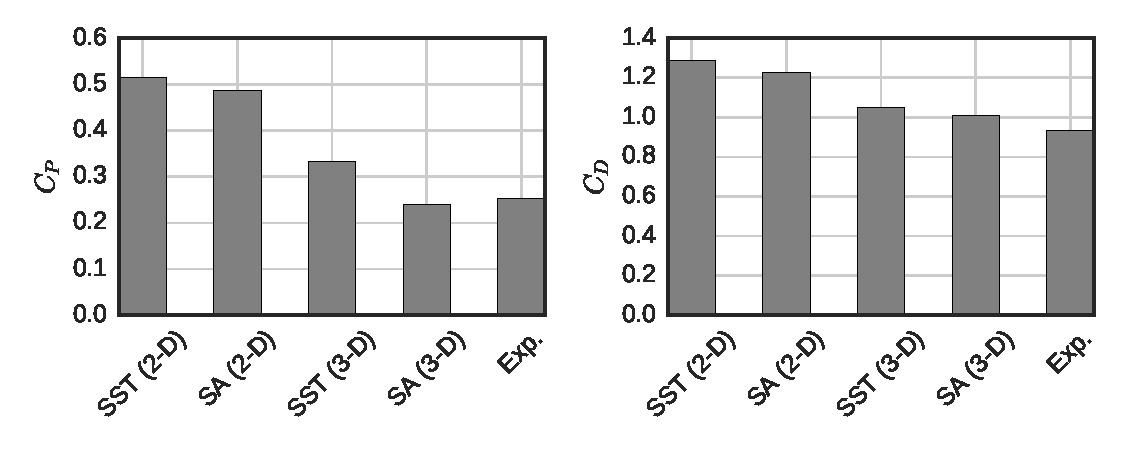
\includegraphics[width=0.9\textwidth]{figures/perf_bar_chart}

    \caption{Power (left) and drag (right) coefficient predictions from
        experiments and each numerical model.}

    \label{fig:perf-comp}
\end{figure}


\subsection{Wake characteristics}

Visualizing the complicated wake generated by the turbine is presented for the
2-D and 3-D Spalart--Allmaras cases in Figure~\ref{fig:vorticity-3D} and
Figure~\ref{fig:vorticity-3D}, respectively. It can be seen how the upstream
blade---as it turns back into the streamwise direction---is shedding a large
amount of spanwise vorticity due to the separated flow. In the 3-D case, strong
tip vortices are also present, which trace the ``contracting'' wake flow on the
$-y$ side of the turbine associated with the induced vertical velocity field.
The 3-D dynamic stall vortex also shows assymmetry about the $x$--$y$ mid-rotor
plane; once again highlighting the importance of three-dimensional effects on
wake dynamics.

\begin{figure}
    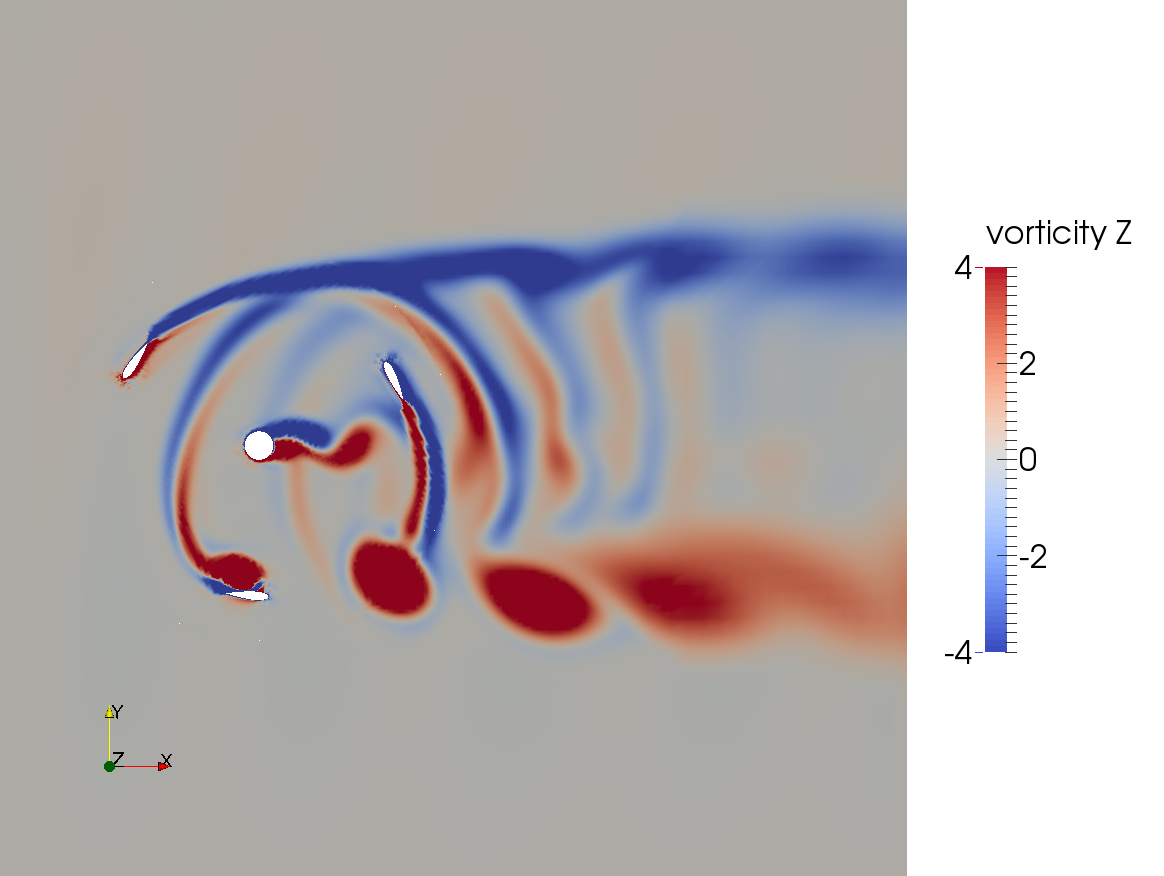
\includegraphics[width=0.65\textwidth]{figures/2D_vorticity_SA_964}
    
    \caption{Instantaneous vorticity contours (at $t=9.64$ s) computed for the
        2-D Spalart--Allmaras case.}
    
    \label{fig:vorticity-2D}
\end{figure}

\begin{figure}
    \centering
    
    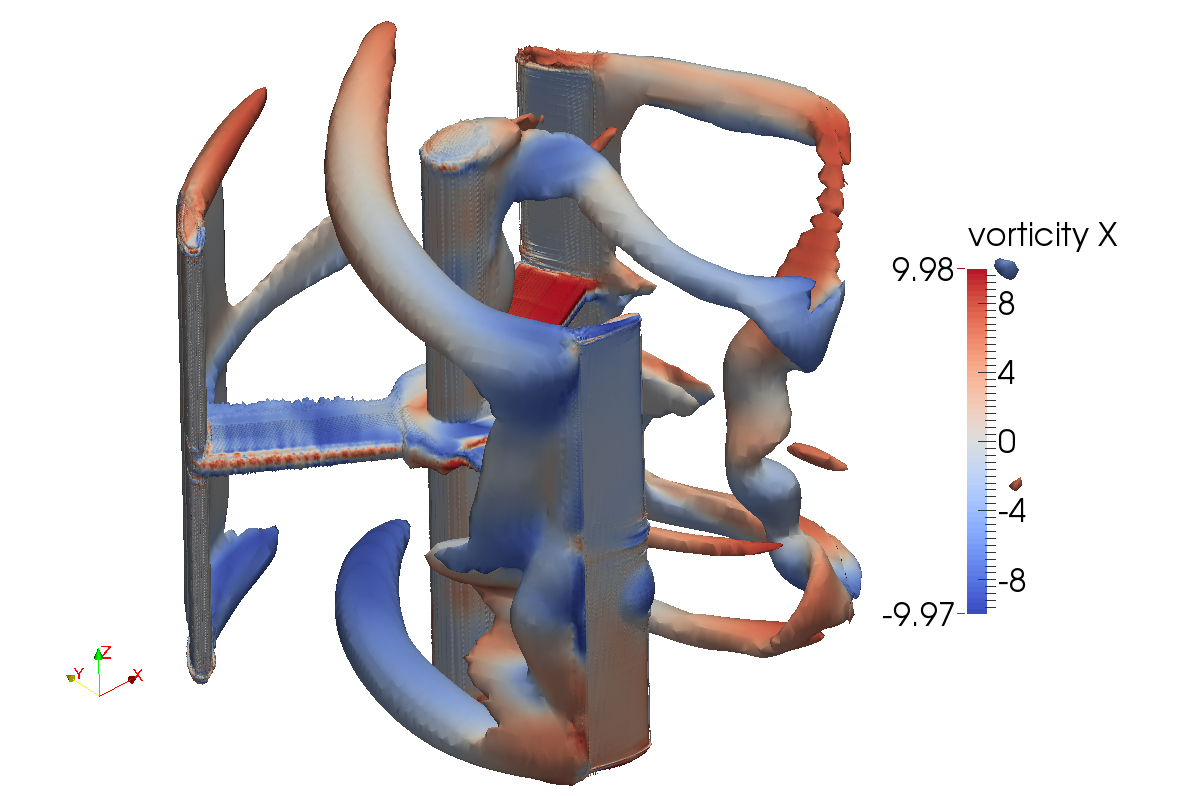
\includegraphics[width=0.8\textwidth]{figures/3D_vorticity_SA_964_10-threshold}
    
    \caption{Iso-vorticity contours (at $t=9.64$ s) colored by the streamwise
        component of vorticity for the 3-D Spalart--Allmaras case.}
    
    \label{fig:vorticity-3D}
\end{figure}


Mean velocity profiles at one turbine diameter downstream are shown in
Figure~\ref{fig:profiles}. The 2-D results suffer from a blockage mismatch, i.e.
keeping the proximity of the walls constant increases the blockage ratio. The
3-D results, however, show good agreement with the experiments.

\begin{figure}
    \centering

    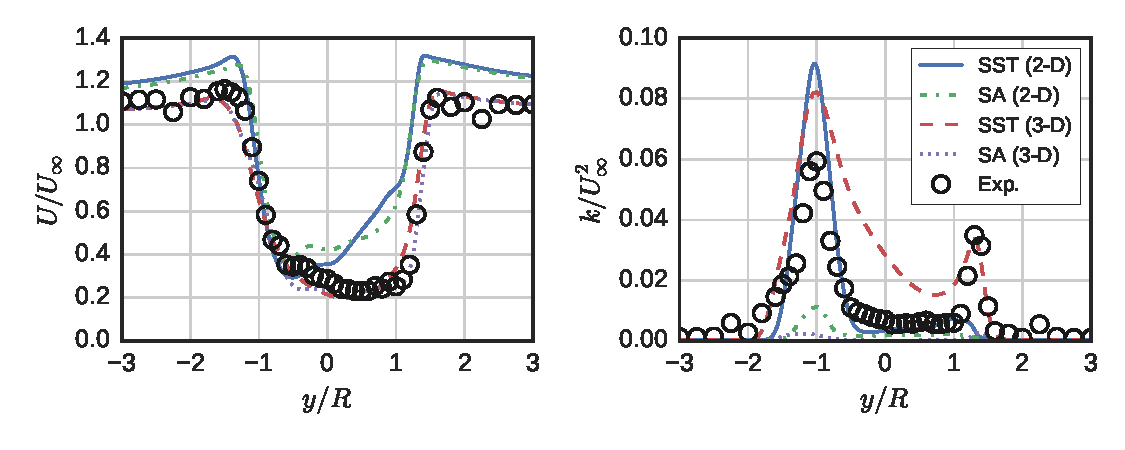
\includegraphics[width=0.95\textwidth]{figures/profiles}

    \caption{Mean velocity (left) and turbulence kinetic energy (right) profiles
        at $x/D=1$ from 2-D simulations, 3-D simulations ($z/H=0$), and experiments
        \cite{Bachant2015-JoT}.}

    \label{fig:profiles}
\end{figure}

Turbulence kinetic energy profiles are also shown in Figure~\ref{fig:profiles}.
The turbulence kinetic energy is calculated as
\begin{equation}
    k = k_{\mathrm{RA}} + \frac{1}{2} \left(
    \overline{U^\prime}^2 +
    \overline{V^\prime}^2 +
    \overline{W^\prime}^2 \right),
    \label{eq:k}
\end{equation}
where $U^\prime = U - \overline{U}$ and $k_{\mathrm{RA}}$ is the kinetic energy
calculated by the turbulence model, which is zero for the SA model. Note that
the statistics of the Reynolds-averaged velocity are calculated from a time
series that has been downsampled to 50 Hz. It is assumed that this is far enough
from the blade passage frequency that differences from the variance in the
original velocity will be negligible.

Both Spalart--Allmaras cases do a poor job predicting the turbulence kinetic
energy in the flow, since it must be resolved as variance in the velocity field.
The 2-D SST model does a good job predicting the peak in $k$ at $y/R=-1$, though
is missing the smaller peak at $y/R=-1$. This is once again likely due to
blockage issues, where local tip speed ratio is decreased, increasing the
blades' instantaneous angle of attack at this location on the downstream
passage. In contrast, the 3-D SST model predicts the $+y$ peak in turbulence
kinetic energy very well, though the $-y$ peak magnitude is overpredicted by
about 30\%. We also see some smearing of $k$ across the center of the rotor,
which is likely due to exaggerated levels of the turbulent eddy viscosity.


\subsubsection{Mean velocity in three dimensions}

In order to visualize the mean velocity field, vector arrows for the mean
cross-stream and vertical components are superimosed on top of contours of the
streamwise component at $X/D=1$ in Figure~\ref{fig:mean-velocity}. Both CFD
models predict the general structure of the mean velocity well, though the SA
case has slightly larger vertical mean flows, which could be due to stronger tip
vortex generation, or lower diffusivity compared with the SST model. Additional
discrepancies between CFD and experiments may be due to the top slip boundary
condition versus the experiment's free surface.

\begin{figure}
    \centering
    \begin{subfigure}[b]{\textwidth}
        \centering 
        
        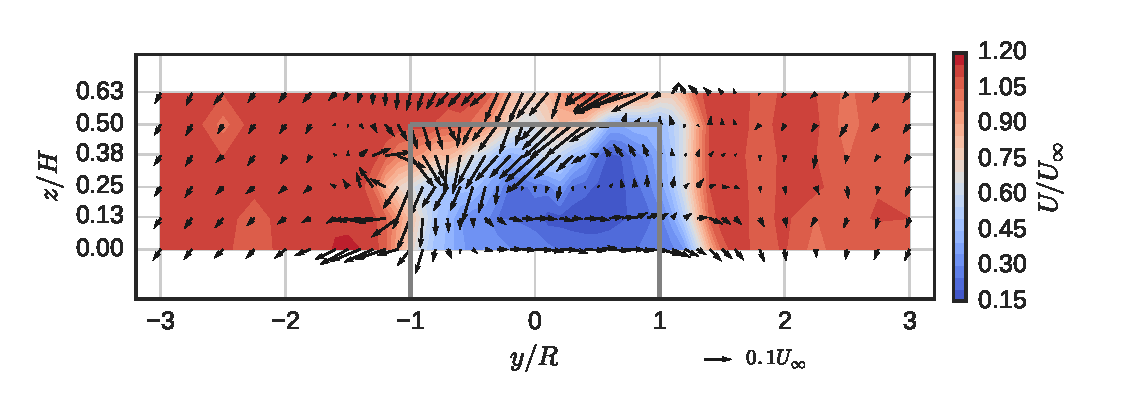
\includegraphics[clip, trim=0 0.1in 0 0.2in,
        width=0.75\textwidth]{figures/meancontquiv_exp}
        
        \caption{Mean velocity field at $x/D=1$ from experiments
            \cite{Bachant2015-RVAT-Re-dep-data}.}
        
        \label{fig:meancontquiv-exp}
    \end{subfigure}

    \begin{subfigure}[b]{\textwidth}
        \centering 
        
        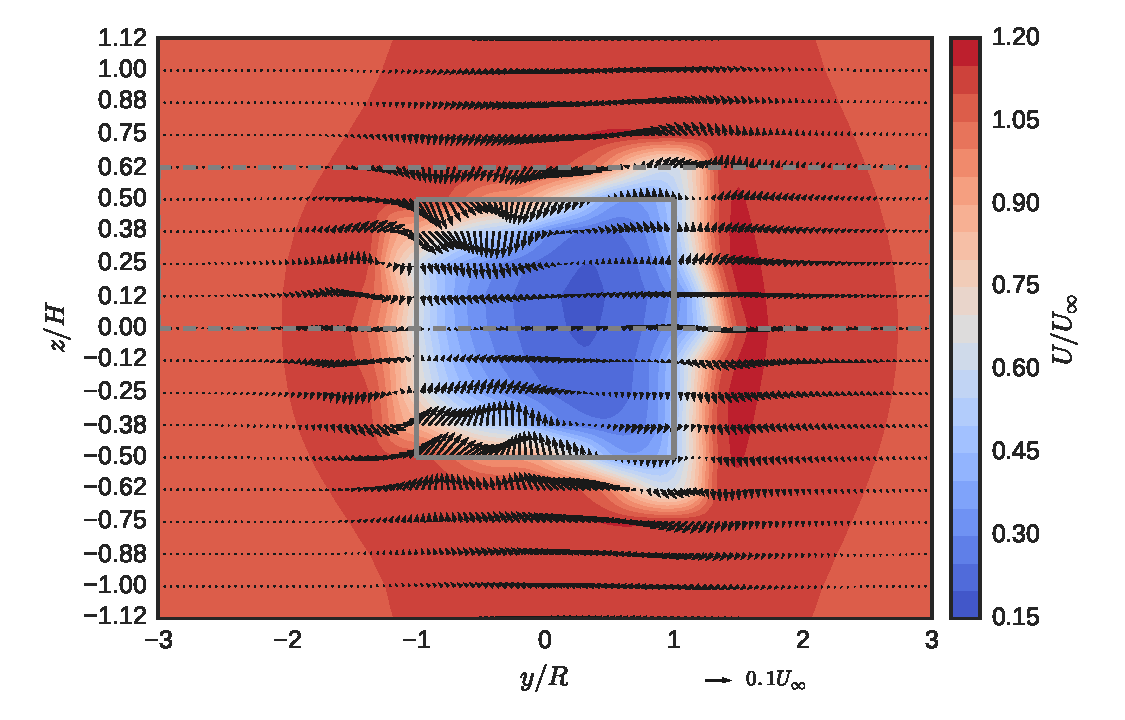
\includegraphics[clip, trim=0 0.2in 0 0.15in,
        width=0.8\textwidth]{figures/meancontquiv_kOmegaSST}
        
        \caption{Mean velocity at $x/D=1$ computed by the 3-D SST model.}
        
        \label{fig:meancontquiv-SST}
    \end{subfigure}

    \begin{subfigure}[b]{\textwidth}
        \centering 
        
        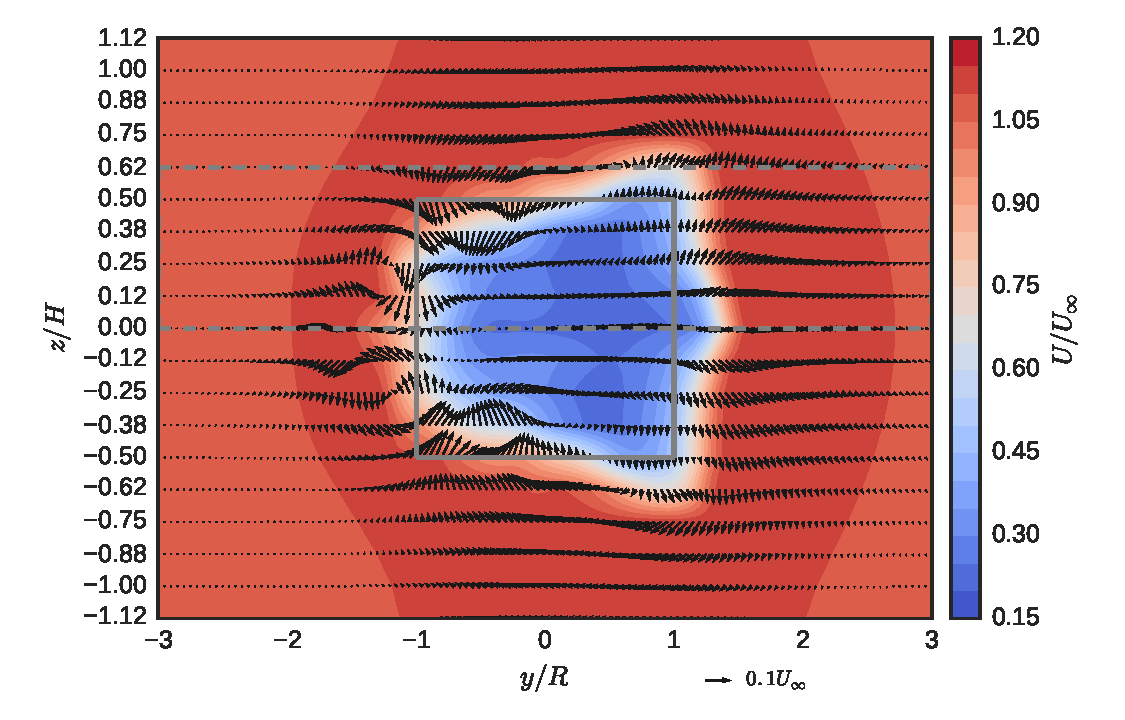
\includegraphics[clip, trim=0 0.2in 0 0.15in,
        width=0.8\textwidth]{figures/meancontquiv_SpalartAllmaras}
        
        \caption{Mean velocity at $x/D=1$ computed by the 3-D SA model.}
        
        \label{fig:meancontquiv-SA}
    \end{subfigure}

    \caption{Mean velocity from experiments and 3-D CFD cases. Solid gray lines
        indicate turbine frontal area and dashed lines indicate experimental
        measurement plane.}
    
    \label{fig:mean-velocity}
\end{figure}


\subsubsection{Turbulence kinetic energy contours}

Turbulence kinetic energy contours for the experimental measurements and each
CFD case at $x/D=1$ are presented in Figure~\ref{fig:kcont}. As seen in the
profiles in Figure\ref{fig:profiles}, the SA model is resolving very little of
the flow unsteadiness. In contrast, the SST model does a good job predicting the
locations and magnitudes of various peaks in $k$. These are generated along the
top of the turbine via tip vortex shedding, and the $-y$ side of the turbine via
dynamic stall. We do however see the smearing effect from the dynamic stall
vortex centered around $z/H=0$, which is likely more of an issue with wake
evolution rather than wake generation.

\begin{figure}
    \centering
    \begin{subfigure}[b]{\textwidth}
        \centering 
        
        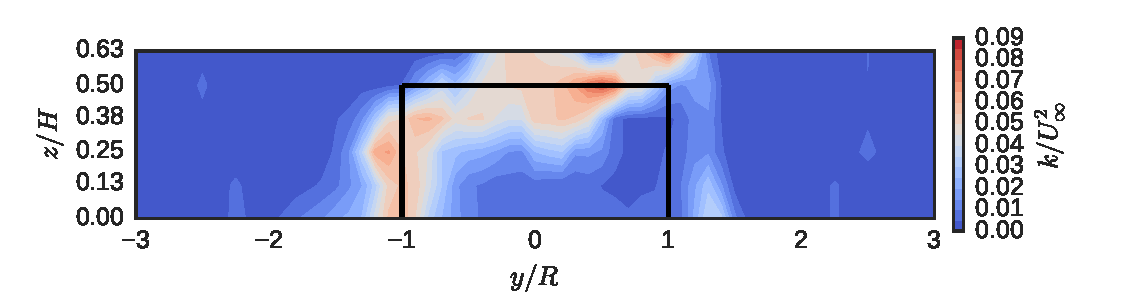
\includegraphics[width=0.95\textwidth]{figures/kcont_exp}
        
        \caption{Turbulence kinetic energy at $x/D=1$ from experiments
            \cite{Bachant2015-RVAT-Re-dep-data}.} 
        
        \label{fig:kcont-exp}
    \end{subfigure}
    
    \begin{subfigure}[b]{\textwidth}
        \centering 
        
        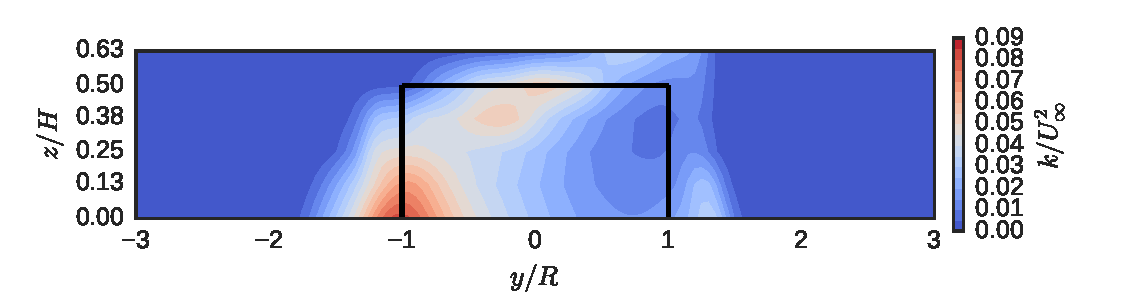
\includegraphics[width=0.95\textwidth]{figures/kcont_kOmegaSST}
        
        \caption{Turbulence kinetic energy at $x/D=1$ computed by the 3-D SST
            model.}
        
        \label{fig:kcont-SST}
    \end{subfigure}
    
    \begin{subfigure}[b]{\textwidth}
        \centering 
        
        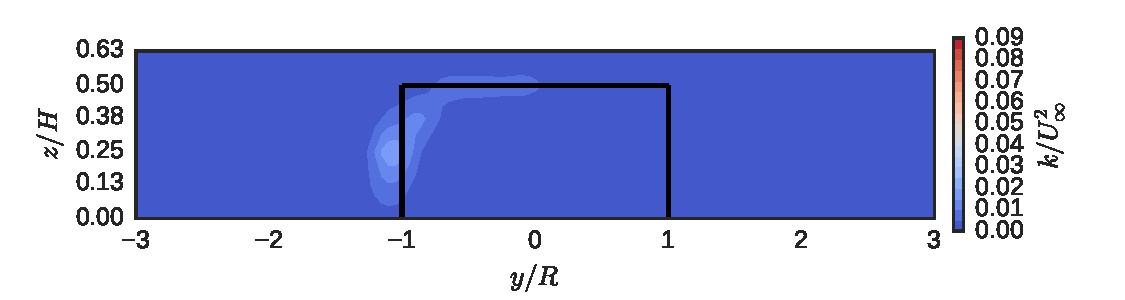
\includegraphics[width=0.95\textwidth]{figures/kcont_SpalartAllmaras}
        
        \caption{Turbulence kinetic energy at $x/D=1$ computed by the 3-D SA
            model.} 
        
        \label{fig:kcont-SA}
    \end{subfigure}
    
    \caption{Turbulence kinetic energy from experiments and 3-D CFD cases. Solid
        black lines indicate turbine frontal area.}
    
    \label{fig:kcont}
\end{figure}

\subsubsection{Momentum recovery}

To get an overall idea of the wake recovery predicted by each model, we
rearrange the streamwise component of the Navier--Stokes equation to isolate
$\partial U / \partial x$---following Bachant and
Wosnik\cite{Bachant2015-JoT}---and compute each term at $X/D = 1$ to compare
with the experimental results.

We use the RANS models' eddy viscosity to calculate the turbulent transport via
\begin{equation}
    \text{Turb. trans.} = \nu_t \nabla^2 \vec{U},
    \label{eq:turb-trans}
\end{equation}
which is a different approach from those taken on the experiments, where Reynolds stresses were measured, but $x$-derivatives were not:
\begin{equation}
    \text{Turb. trans. (exp.)} = 
    -\left( 
    \frac{\partial}{\partial y} \overline{u^\prime v^\prime}
    +
    \frac{\partial}{\partial z} \overline{u^\prime w^\prime}
    \right).
\end{equation}
As such, we should not be surprised if the CFD models predict higher levels of
turbulent transport than the experiments.

Normalized weighted averages for each recovery term at $x/D=1$ are computed and
multiplied by the cross-sectional area of the measurement plane, or the channel
width in the 2-D cases. Results are shown in a bar chart in
Figure~\ref{fig:recovery}. Consistent with the relatively large Reynolds number
regime, viscous transport is essentially negligible compared with other
mechanisms. Cross-stream advection---or the tendency of streamlines to diverge
and reduce the streamwise momentum---produces a negative effect for all cases,
though the 3-D SST model predicts significantly lower values. Vertical advection
is by definition zero for the 2-D cases. The 3-D cases show varying
results---with the SST model overpredicting and SA underpredicting the vertical
velocity's effect on replenishing streamwise momentum.

Turbulent transport and streamwise pressure gradient terms show the largest
discrepancy between results. The 3-D SST case, despite doing a good job
predicting turbulence kinetic energy, significantly overpredicts the turbulent
transport term, while other CFD cases are comparable with the experiment. This
seems to be balanced by a large adverse pressure gradient, which is also present
to a smaller degree in the 3-D SA case. Interestingly, in contrast, both 2-D CFD
cases create a wake where the pressure gradient is acting to accelerate the flow
at $x/D=1$. Unfortunately, pressure data were not acquired from the experiment,
though the 3-D delayed detached eddy simulation (DDES) of Boudreau and Dumas
\cite{Boudreau2015} concur with the adverse pressure gradient condition.

\begin{figure}[ht]
    \centering

    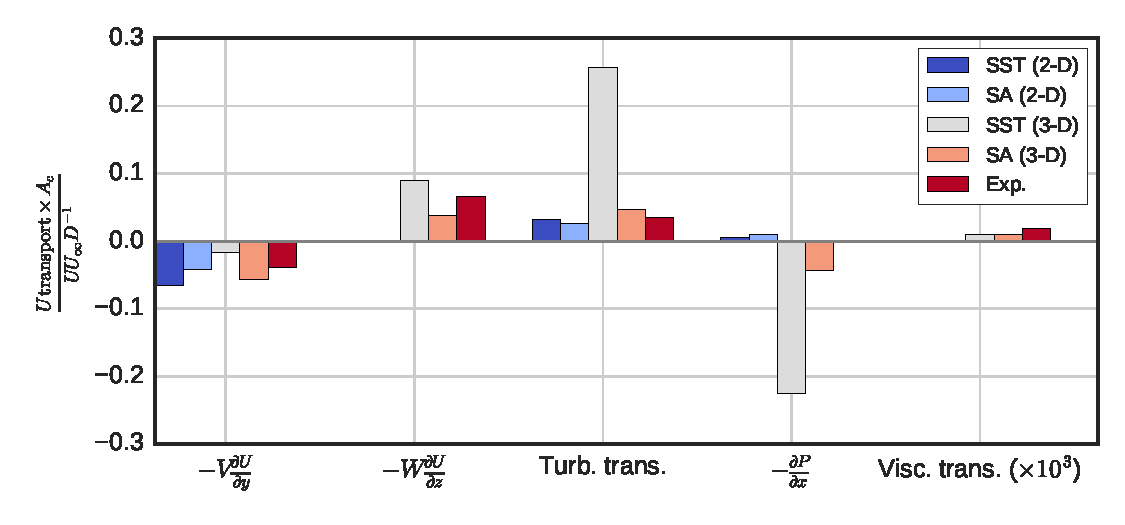
\includegraphics[width=0.9\textwidth]{figures/mom_bar_graph}

    \caption{Weighted sum normalized momentum recovery terms for each CFD case
        and experiments\cite{Bachant2015-RVAT-Re-dep-data} at $x/D=1$.}

    \label{fig:recovery}
\end{figure}


\section{Conclusions}

A cross-flow turbine was modeled using the $k$--$\omega$ SST and
Spalart--Allmaras Reynolds-averaged Navier--Stokes turbulence models to test
their abilities to predict turbine performance and near-wake dynamics. It was
observed that when modeled in 2-D, the performance is over-predicted compared to
the data from the tow tank experiments, which was expected due to omission of
blade end effects, support strut drag, and increased blockage. Vertical (or
axial) wake dynamics were unresolved in the 2-D model, despite being identified
as a significant contributor to streamwise wake recovery, which casts doubt on
the 2-D model's applicability as a tool to study array spacing effects.

These results may also help develop new tip loss corrections for blade element
type models, which currently only exist for axial-flow rotors.


\begin{acknowledgments}
    The authors would acknowledge funding through a National Science Foundation
    CAREER award (principal investigator Martin Wosnik, NSF 1150797, Energy for
    Sustainability, program manager Gregory L. Rorrer). The authors also thank
    Dr. Vincent S. Neary and the Sandia National Laboratories Water Power
    Program for use of their Red Mesa high performance computing cluster.
\end{acknowledgments}

% Create the reference section using BibTeX:
\bibliography{library}

\end{document}
